\documentclass[a4paper,12pt]{article}
\usepackage[utf8]{inputenc}
\usepackage[german]{babel}
\usepackage{amsmath}
\usepackage{amsfonts}
\usepackage{amssymb}
\usepackage{tikz-cd}
\usepackage{lmodern}
\usepackage{bbold}
\usepackage{float}
\usepackage{graphicx}
\usepackage{hyperref}
\usepackage[left=3cm,right=3cm,top=2cm,bottom=2cm]{geometry}
\usepackage{framed}
\usepackage{marginnote}
\title{Lie-Algebren (Vortrag am 5. Juni)}
\author{Philipp Arras}

\usepackage{scrpage2}
\pagestyle{scrheadings}
\clearscrheadfoot
\ohead{\pagemark}
\ihead{Lie-Algebren (Vortrag am 5. Juni)}
\ifoot{\today}
\ofoot{Philipp Arras}
\setheadtopline{1pt} \setheadsepline{0.4pt}
\setfootsepline{0.4pt} \setfootbotline{1pt}

\begin{document}
\maketitle
\setcounter{section}{-1}
\section{Vorbemerkungen}
%\subsection{Motivation}
%\emph{Warum beschäftigen wir uns überhaupt mit Lie-Algebren?}\\
%Lie-Algebren treten sowohl in der Mathematik als auch in der Physik oft auf:
%\begin{itemize}
%\item Natürlich haben wir $\mathfrak{gl}(V)$ mit $[A,B] = AB-BA$
%\item Man kann jede assoziative Algebra $A$ zu einer Lie-Algebra machen: $[x,y] = x\cdot y-y\cdot x$\footnote{Andersrum kann man jede Lie-Algebra in eine assoziative Algebra mit Kommutator einbetten. Dies wird in späteren Vorträgen gezeigt.}
%\item Die glatten Vektorfelder auf einer differenzierbaren Mannigfaltigkeit zusammen mit der Lie-Klammer bilden eine unendlichdimensionale Lie-Algebra
%\item In der Physik sind Lie-Algebren wichtig, weil sie als Tangentialräume am Einselement von Lie-Gruppen auftreten. Zum Beispiel beschreibt die Gruppe $SO(3)$ die Drehungen im 3-dimensionalen Raum. Lie-Gruppen beschreiben kontinuierliche Symmetrien und die zugehörige Lie-Algebra ist der Vektorraum der infinitesimalen Symmetrietransformationen. Von der Lie-Algebra kommt man über die Exponentialfunktion zur Lie-Gruppe zurück.
%\end{itemize}

\subsection{Setup}
Sei $L$ halbeinfache Lie-Algebra über einem abgeschlossenen Körper der Charakteristik Null. Sei $H$ eine maximale torische Unteralgebra.

Im Vortrag von Dr. Kasten wurde folgende Abbildung beschrieben:
\begin{align*}
(L,H) \mapsto (E,\Phi)
\end{align*}
wobei $E$ ein euklidischer Vektorraum und $ \Phi$ ein Wurzelsystem ist. Wir klassifizieren jetzt die Paare $(E,\Phi)$. Im nächsten Vortrag werden wir sehen, dass obige Abbildung bijektiv und die Wahl von $H$ nicht entscheidend ist. 

\subsection{Bezeichnungen}
Im Folgenden sei immer $\Phi$ ein Wurzelsystem vom Rang $l$ in einem euklidischen Raum $E$ mit Weyl-Gruppe $\mathcal{W}$ und $\Delta$ eine Basis von $\Phi$.
\marginnote{3 min}
\setcounter{section}{9}
\section{Einfache Wurzeln und die Weyl-Gruppe}
\setcounter{subsection}{3}
\subsection{Irreduzible Wurzelsysteme}
\paragraph{Definition (irreduzible Wurzelsysteme)} Wir nennen $\Phi$ irreduzibel, wenn es nicht in zwei echte zueinander orthogonale Teilmengen zerlegt werden kann, d.h. dass jede Wurzel der einen Teilmenge orthogonal auf jeder Wurzel der anderen Teilmenge steht.\\
Beispiel: $A_1 \times A_1$ ist reduzibel. $A_2$ ist irreduzibel.

\paragraph{Bemerkung} $\Phi$ ist irreduzibel $\Leftrightarrow$ $\Delta$ ist irreduzibel.\\
\glqq $\Leftarrow$\grqq: Beweis durch Kontraposition. Sei $\Phi = \Phi_1 \cup \Phi_2$ nicht irreduzibel, also reduzibel. Wenn $\Delta$ nicht komplett in einer der Teilmengen enthalten ist, induziert die Zerlegung eine Zerlegung von $\Delta$. Wenn aber $\Delta \subset \Phi_1$, folgt $0 = (\Delta,\Phi_2) = (E, \Phi_2)$, weil $\Delta$ Basis von $E$ ist.  $\Delta$ kann also nicht komplett in $\Phi_1$ liegen.

\glqq $\Rightarrow$\grqq: Sei $\Phi$ irreduzibel, aber $\Delta$ nicht: $\Delta = \Delta_1 \cup \Delta_2$ mit $(\Delta_1,\Delta_2) = 0$. Theorem 10.3(c) besagt, dass jede Wurzel zu einer einfachen Wurzel konjugiert ist (über die Weylgruppe)\\
$\Rightarrow \quad \Phi = \Phi_1 \cup \Phi_2$ mit $\Phi_i = \{ \alpha \in \Phi \;|\; \alpha \text{ ist konjugiert zu einem } \alpha' \in \Delta_i\}$. Dies ist wegen der Definition von Basis wohldefiniert. \\
Wir wissen: $(\alpha,\beta)=0 \Rightarrow [\sigma_\alpha, \sigma_\beta] = 0$. Weil $\mathcal{W}$ von den einfachen Spiegelungen $\sigma_\alpha, \alpha \in \Delta$ erzeugt wird, kann jede Wurzel aus $\Phi_i$ aus einer Summe oder Differenz von Elementen aus $\Delta_i$ geschrieben werden.\\
$\Rightarrow\quad \Phi_i \subset E_i \equiv \text{span}(\Delta_i)$. Damit sehen wir, dass $(\Phi_1,\Phi_2)=0$. Weil $\Phi$ irreduzibel ist, folgt: $\Phi_1 = \varnothing$ oder $\Phi_2 = \varnothing $ \\
$\Rightarrow\quad \Delta_1=\varnothing$ oder $\Delta_2 = \varnothing$.
\hfill$\Box$
\marginnote{11 min}

\paragraph{Lemma 1} \emph{Sei $\Phi$ irreduzibel. (1) Bezüglich der partiellen Ordnung\footnote{$\Delta$ definiert $\prec$: $\mu \prec \lambda :\Leftrightarrow \mu -\lambda$ ist Summe von (positiven=einfachen) Wurzeln oder $\lambda= \mu$.\\Eine partielle Ordnung ist transitiv, reflexiv und antisymmetrisch (nicht total)}
 $\prec$ gibt es eine eindeutig bestimmte maximale Wurzel $\beta$. (2) Wenn $\beta = \sum k_\alpha \alpha, \alpha \in \Delta \quad \Rightarrow \quad k_\alpha>0$}\\
Beweis von (2): Sei $\beta = \sum k_\alpha \alpha$ maximal bezüglich der Ordnung, also $\beta \succ 0$.\\
Sei $\Delta_1 = \{ \alpha \in \Delta | k_\alpha >0 \}$ und $\Delta_2 = \{ \alpha \in \Delta | k_\alpha = 0 \}$. Dann gilt: $\Delta = \Delta_1 \cup \Delta_2$.\\
Angenommen $\Delta_2 \neq \varnothing$. Es gilt: $(\alpha,\beta) \leq 0\; \forall \alpha\in\Delta_2$ (Lemma 10.1).\\
Weil $\Phi$ irreduzibel ist, muss mindestens ein $\alpha \in\Delta_2$ nicht-orthogonal zu $\Delta_1$ sein: $(\alpha,\alpha') \overset{\text{10.1}}{<} 0 , \alpha'\in\Delta_1$. Damit ist $(\alpha,\beta) <0$. Aus Lemma 9.4 folgt, dass $\alpha+\beta$ eine Wurzel ist. Dies ist ein Widerspruch zur Annahme, dass $\beta$ maximal ist. Damit ist $\Delta_2 = \varnothing, k_\alpha>0$. Außerdem haben wir damit gezeigt, dass $(\alpha,\beta) \geq 0\;\forall \alpha\in\Delta$ und $(\alpha,\beta)>0$ für mindestens ein $\alpha$, weil $E = \text{span}(E)$.\\
Beweis von (1): Sei $\beta'$ eine weitere maximale Wurzel. Wie wir gerade gesehen haben, gilt $(\alpha,\beta)>0$ für mindestens ein $\alpha\in\Delta$.\\
 $\Rightarrow\quad (\beta,\beta')>0 \quad \Rightarrow\quad \beta-\beta'$ ist eine Wurzel, solange nicht $\beta= \beta'$. Aber wenn $\beta-\beta'$ eine Wurzel ist, muss entweder $\beta \succ \beta'$ oder $\beta' \succ \beta$. Beides führt unmittelbar zum Widerspruch.
 \hfill$\Box$
\marginnote{18 min}

\paragraph{Lemma 2} \emph{Sei $\Phi$ irreduzibel. Dann operiert $\mathcal{W}$ irreduzibel auf $E$, d.h. außer $E$ und ${0}$ gibt es keine $\mathcal{W}$-invarianten Unterräume. Insbesondere spannt der $\mathcal{W}$-Orbit einer Wurzel ganz $E$ auf.} \\
Es ist klar, dass die zweite Aussage aus der Ersten folgt. Wir zeigen also den ersten Teil.\\
Sei $\varnothing \neq E' \subset E$ ein $\mathcal{W}$-invarianter Teilraum. Das orthogonale Komplement $E''$ ist natürlich ebenfalls $\mathcal{W}$-invariant.\\
Jedes $\alpha\in\Phi$ liegt entweder in $E'$ oder $E'$ liegt in $P_\alpha$, weil $\sigma_\alpha (E')=E'$.\\
$\alpha \notin E' \Rightarrow \alpha \in E'' $. Jede Wurzel liegt also entweder in dem einen oder dem anderen Unterraum. Weil $\Phi\; E$ erzeugt, folgt $E'=E$.
\hfill$\Box$ 
\marginnote{20 min}

\paragraph{Lemma 3} \emph{Sei $\Phi$ irreduzibel. Dann (1) existieren höchstens zwei Wurzellängen in $\Phi$ und (2) alle Wurzeln einer bestimmten Länge sind konjugiert unter $\mathcal{W}$.}\\
Seien $\alpha,\beta$ beliebige Wurzeln.\\
Nicht alle $\sigma(\alpha)\; (\sigma \in\mathcal{W})$ können orthogonal zu $\beta$ sein, weil $E=\underset{\sigma\in\mathcal{W}}{\text{span}}(\sigma(\alpha))$.\\
(1 mündlich): Wenn $(\alpha,\beta)\neq 0$ wissen wir (aus Abschnitt 9.4), dass alle Verhältnisse von quadrierten Wurzellängen $1,2,3,1/2$ oder $1/3$ sein müssen. Gäbe es drei unterschiedliche Wurzellängen, würde u.a. das Verhältnis $3/2$ auftreten.\hfill \#\\
(2): Seinen nun $\alpha, \beta$ Wurzeln gleicher Länge. Wir können OE annehmen, dass sie nichtorthogonal sind (ersetze eine Wurzel durch eine $\mathcal{W}$-Konjugierte) und verschieden (sonst sind wir schon fertig).\\
$\overset{(9.4)}{\Rightarrow}$ $\langle\alpha,\beta\rangle = \langle\beta,\alpha\rangle=\pm 1$. Falls nötig ersetzen wir $\beta \rightarrow -\beta = -\sigma_\beta(\beta)$\footnote{auch hier wird wieder ein Element von $\mathcal{W} $ angewendet}, sodass $\langle\alpha,\beta\rangle = 1$.\\
Aus $\sigma_\alpha(\beta) = \beta - \frac{2(\beta,\alpha)}{(\alpha,\alpha)}\,\alpha$ folgt $(\sigma_\alpha \sigma_\beta \sigma_\alpha)(\beta)= \sigma_\alpha \sigma_\beta (\beta-\alpha) = \sigma_\alpha (- \beta-\alpha+\beta) = \alpha$
\hfill$\Box$
\marginnote{24 min}

\paragraph{Definition} Sei $\Phi$ irreduzibel. Haben wir zwei Wurzellängen, sprechen wir von kurzen und von langen Wurzeln. Haben alle Wurzeln gleiche Länge, nennen wir sie lang.

\paragraph{Lemma 4} \emph{Sei $\Phi$ irreduzibel mit zwei unterschiedlichen Wurzellängen. Dann ist die maximale Wurzel aus Lemma 1 eine lange Wurzel.}\\
Sei $\alpha\in\Phi$. Es reicht z.z, dass $(\beta,\beta) \geq (\alpha,\alpha)$.\\
Ersetze $\alpha$ durch eine $\mathcal{W}$-Konjugierte, die im Abschluss der zu $\Delta$ fundamentalen Weyl-Kammer liegt. Weil $\beta-\alpha \succ 0$ (Lemma 1)\footnote{Warum?}, gilt $(\gamma, \beta-\alpha) \geq 0\quad \forall \gamma \in \overline{\mathcal{C}(\Delta)}$. setze $\gamma = \beta$ und $\gamma = \alpha$.\\
$\Rightarrow\quad (\beta, \beta) \geq (\beta,\alpha)\geq (\alpha,\alpha)$.
\hfill$\Box$ 
\marginnote{27 min}

\section{Klassifikation}
\subsection{Cartan-Matrix von $\Phi$}
\paragraph{Definition (Cartan Matrix)} Sei $(\alpha_1 , \ldots , \alpha_l)$ eine geordnete Liste der einfachen Wurzeln. Wir nennen $(\langle \alpha_i , \alpha_j \rangle)_{ij}$ \emph{Cartan-Matrix} von $\Phi$.

\paragraph{Bemerkungen}
\begin{itemize}
\item Diese Definition ist abhängig von der Ordnung der einfachen Wurzeln.
\item Die Cartan-Matrix ist unabhängig von der Wahl von $\Delta$ (folgt aus Theorem 10.3(b)).
\item Die Cartan-Matrix ist nichtsingulär (folgt aus Abschnitt 8.5).
\item Wir werden sehen, dass die Cartan-Matrix $\Phi$ komplett charakterisiert.
\item Sei $(\Phi' \subset E' , \Delta')$ ein weiteres Wurzelsystem mit Basis $\Delta'$. Wenn $\langle \alpha_i, \alpha_j\rangle = \langle \alpha'_i, \alpha'_j \rangle$ für $1 \leq i,j,\leq l$, dann gilt:\\
Die Abbildung  $\Psi: \alpha_i \mapsto \alpha'_i$ ist ein VR-Isomorphismus mit:
	\begin{itemize}
	\item $\Psi: \Phi \twoheadrightarrow \Phi'$
	\item $\langle \Psi (\alpha), \Psi (\beta) \rangle = \langle\alpha,\beta\rangle \quad \forall \alpha, \beta \in \Phi$
	\end{itemize}
Damit können wir im Prinzip aus der Cartan-Matrix $\Phi$ bestimmen.\footnote{s. Seite 56}
\paragraph{Beweis:}\
\begin{itemize}
\item \emph{$\Psi$ existiert und ist eindeutig:}\\ $\lbrace \begin{array}{c}
\Delta \\ 
\Delta'
\end{array} \rbrace$ ist Basis von $\lbrace \begin{array}{c}
E \\ 
E'
\end{array} \rbrace$
$\Rightarrow \exists !$ VR-Isomorphismus $\Psi: E \rightarrow E'$ mit $\Psi (\alpha_i) = \alpha'_i \quad \forall i$.

\item \emph{Folgendes Diagramm kommutiert: }\\
 \begin{tikzcd}
  E \arrow{d}[swap]{\sigma_\alpha} \arrow{r}{\Psi} & E' \arrow{d}{ \sigma_{\Psi(\alpha)}} \\
  E \arrow{r}{\Psi}                             & E' \\
\end{tikzcd}\\
%\emph{Es gilt: $\sigma_{\Psi(\alpha)} \circ \Psi = \Psi \circ \sigma_\alpha$:}\\
Es gilt: 
	\begin{align*}
	\sigma_{\Psi(\alpha)}(\Psi(\beta)) &= \sigma_{\alpha'} (\beta')\\
	&= \beta'-\langle\beta',\alpha'\rangle\alpha'\\
	&=\Psi (\beta) - \langle\beta,\alpha\rangle\Psi (\alpha)\\
	&= \Psi (\beta - \langle\beta,\alpha\rangle \alpha)\\
	&= \Psi (\sigma_\alpha (\beta))
	\end{align*}
	\item \emph{$\Psi$ bildet $\Phi$ surjektiv auf $\Phi'$ab.} \\
Die Weyl-Gruppen $\mathcal{W}, \mathcal{W}'$ werden von einfachen Spiegelungen erzeugt.\\
$ \overset{\text{Theorem 10.3(d)}}{\Longrightarrow} \xi_\Psi: \mathcal{W} \rightarrow \mathcal{W'},\, \sigma \mapsto \Psi\circ\sigma\circ\Psi^{-1}$ ist ein Gruppen-Isomorphismus mit $\xi_\Psi (\sigma_\alpha) = \sigma_{\Psi(\alpha)} \quad \alpha \in \Delta$ (folgt aus dem kommutativen Diagramm).\\
Weil jedes $\beta\in\Phi$ zu einem $\alpha\in\Delta$ konjugiert ist (also $\exists \sigma\in\mathcal{W}:\: \sigma (\alpha)=\beta$, Theorem 10.3(c)), gilt
\begin{align*}
\Psi(\beta) = \Psi(\sigma(\alpha)) = (\Psi\circ\sigma\circ\Psi^{-1} )(\Psi(\alpha)) \in \Phi'
\end{align*}
Lassen wir $\sigma\in\mathcal{W}$ und $\alpha\in\mathcal{W}$ laufen, erreichen wir ganz $\Phi'$. Also:
\begin{align*}
\Psi: \Phi \twoheadrightarrow \Phi'
\end{align*}

\marginnote{36 min}
\item \emph{Die Cartan-Zahlen bleiben unter $\Psi$ erhalten.}\\
Seien $\alpha,\beta\in\Phi$ und $\sigma,\tau\in\mathcal{W}$, s.d. $\alpha=\sigma(\alpha_i),\beta=\tau(\alpha_j)$ mit $\alpha_i,\alpha_j \in\Delta$.\\
Dann gilt: 
\begin{align*}
\langle\alpha,\beta\rangle &= \langle \sigma(\alpha_i),\tau(\alpha_j) \rangle\\
&\overset{\text{Lemma 9.2}}{=} \langle \underbrace{ \tau^{-1} \sigma(\alpha_i)}_{=\sum_k c_k \alpha_k},\alpha_j \rangle\\
&= \sum_k c_k \langle\alpha_k,\alpha_j\rangle\\
&\overset{\text{Vor.}}{=} \sum_k c_k \langle\Psi(\alpha_k),\Psi(\alpha_j)\rangle\\
&= \langle \Psi(\tau^{-1}\sigma(\alpha_i)),\Psi(\alpha_j)\rangle\\
&= \langle \tau^{-1}\Psi(\sigma(\alpha_i)),\Psi(\alpha_j)\rangle\\
&= \langle \Psi(\sigma(\alpha_i)),\tau\Psi(\alpha_j)\rangle\\
&= \langle \Psi(\sigma(\alpha_i)),\Psi(\tau(\alpha_j))\rangle\\
&= \langle\Psi(\alpha),\Psi(\beta)\rangle
\end{align*}


\end{itemize}
\hfill $\Box$\\



\end{itemize}
\marginnote{39 min}


\subsection{Coxeter-Graphen und Dynkin-Diagramme}
Seien $\alpha, \beta$ zwei positive Wurzeln. Dann gilt: $\langle \alpha, \beta\rangle\langle\beta, \alpha\rangle = 0,\, 1,\, 2 \text{ oder } 3$ (Abschnitt 9.4). Wir betrachten ab jetzt nur noch positive Wurzeln, weil $\Phi^- = -\Phi^+$ und wir deshalb schon alle Wurzeln beschrieben haben, wenn wir die positiven Wurzeln beschrieben haben.\\
Zur besseren Anschaulichkeit folgende Definition.
\paragraph{Definition (Coxeter Graph)} Der Coxeter Graph von $\Phi$ ist ein Graph mit $l$ Vertices, wobei die $i$te und die $j$te Vertex ($i\neq j$) durch $\langle \alpha_i, \alpha_j\rangle\langle\alpha_j, \alpha_i\rangle$ Kanten verbunden sind.

\paragraph{Bemerkung:}
Wenn alle Wurzeln gleiche Länge haben, gilt $\langle \alpha_i, \alpha_j\rangle = \langle \alpha_j, \alpha_i\rangle$. Deshalb sind durch den Coxeter-Graph alle Cartan-Zahlen bestimmt.\\
Haben die Wurzeln unterschiedliche Länge, funktioniert das nicht mehr. In diesem Fall erweitern wir unsere Definition.
\paragraph{Definition (Dynkin-Diagramm)}
Ein Dynkin-Diagramm ist ein Coxeter-Graph, bei dem an jeder Kante, die zwischen Wurzeln unterschiedlicher Länge liegt, ein Pfeil hinzugefügt wird, der von der langen zur kurzen Wurzel zeigt.\footnote{Im Buch wird dies am Beispiel von $F_4$ vorgeführt: S. 57}
\marginnote{42 min}

\subsection{Irreduzible Komponenten}
Wie wir in Abschnitt 10.4 gesehen haben, ist $\Phi$ irreduzibel genau dann wenn $\Phi$ (oder äquivalent $\Delta$) nicht in zwei echte orthogonale Teilmengen aufgeteilt werden kann. Dies ist offensichtlich genau dann der Fall, wenn der Coxeter Graph im gewöhnliche Sinne zusammenhängend ist.\footnote{Hier fehlt noch was, wobei mir noch nicht klar ist, wofür man das braucht.}

\subsection{Klassifikationssatz}
Wir wir gerade gesehen haben, reicht es irreduzible Wurzelsysteme, also zusammenhängende Dynkin-Diagramme zu betrachten.

\subsubsection*{Theorem}
Sei $\Phi$ ein irreduzibles Wurzelsystem vom Rang $l$. Dann ist sein Dynkin-Diagramm eines der Folgenden:

\begin{figure}[H]
\centering
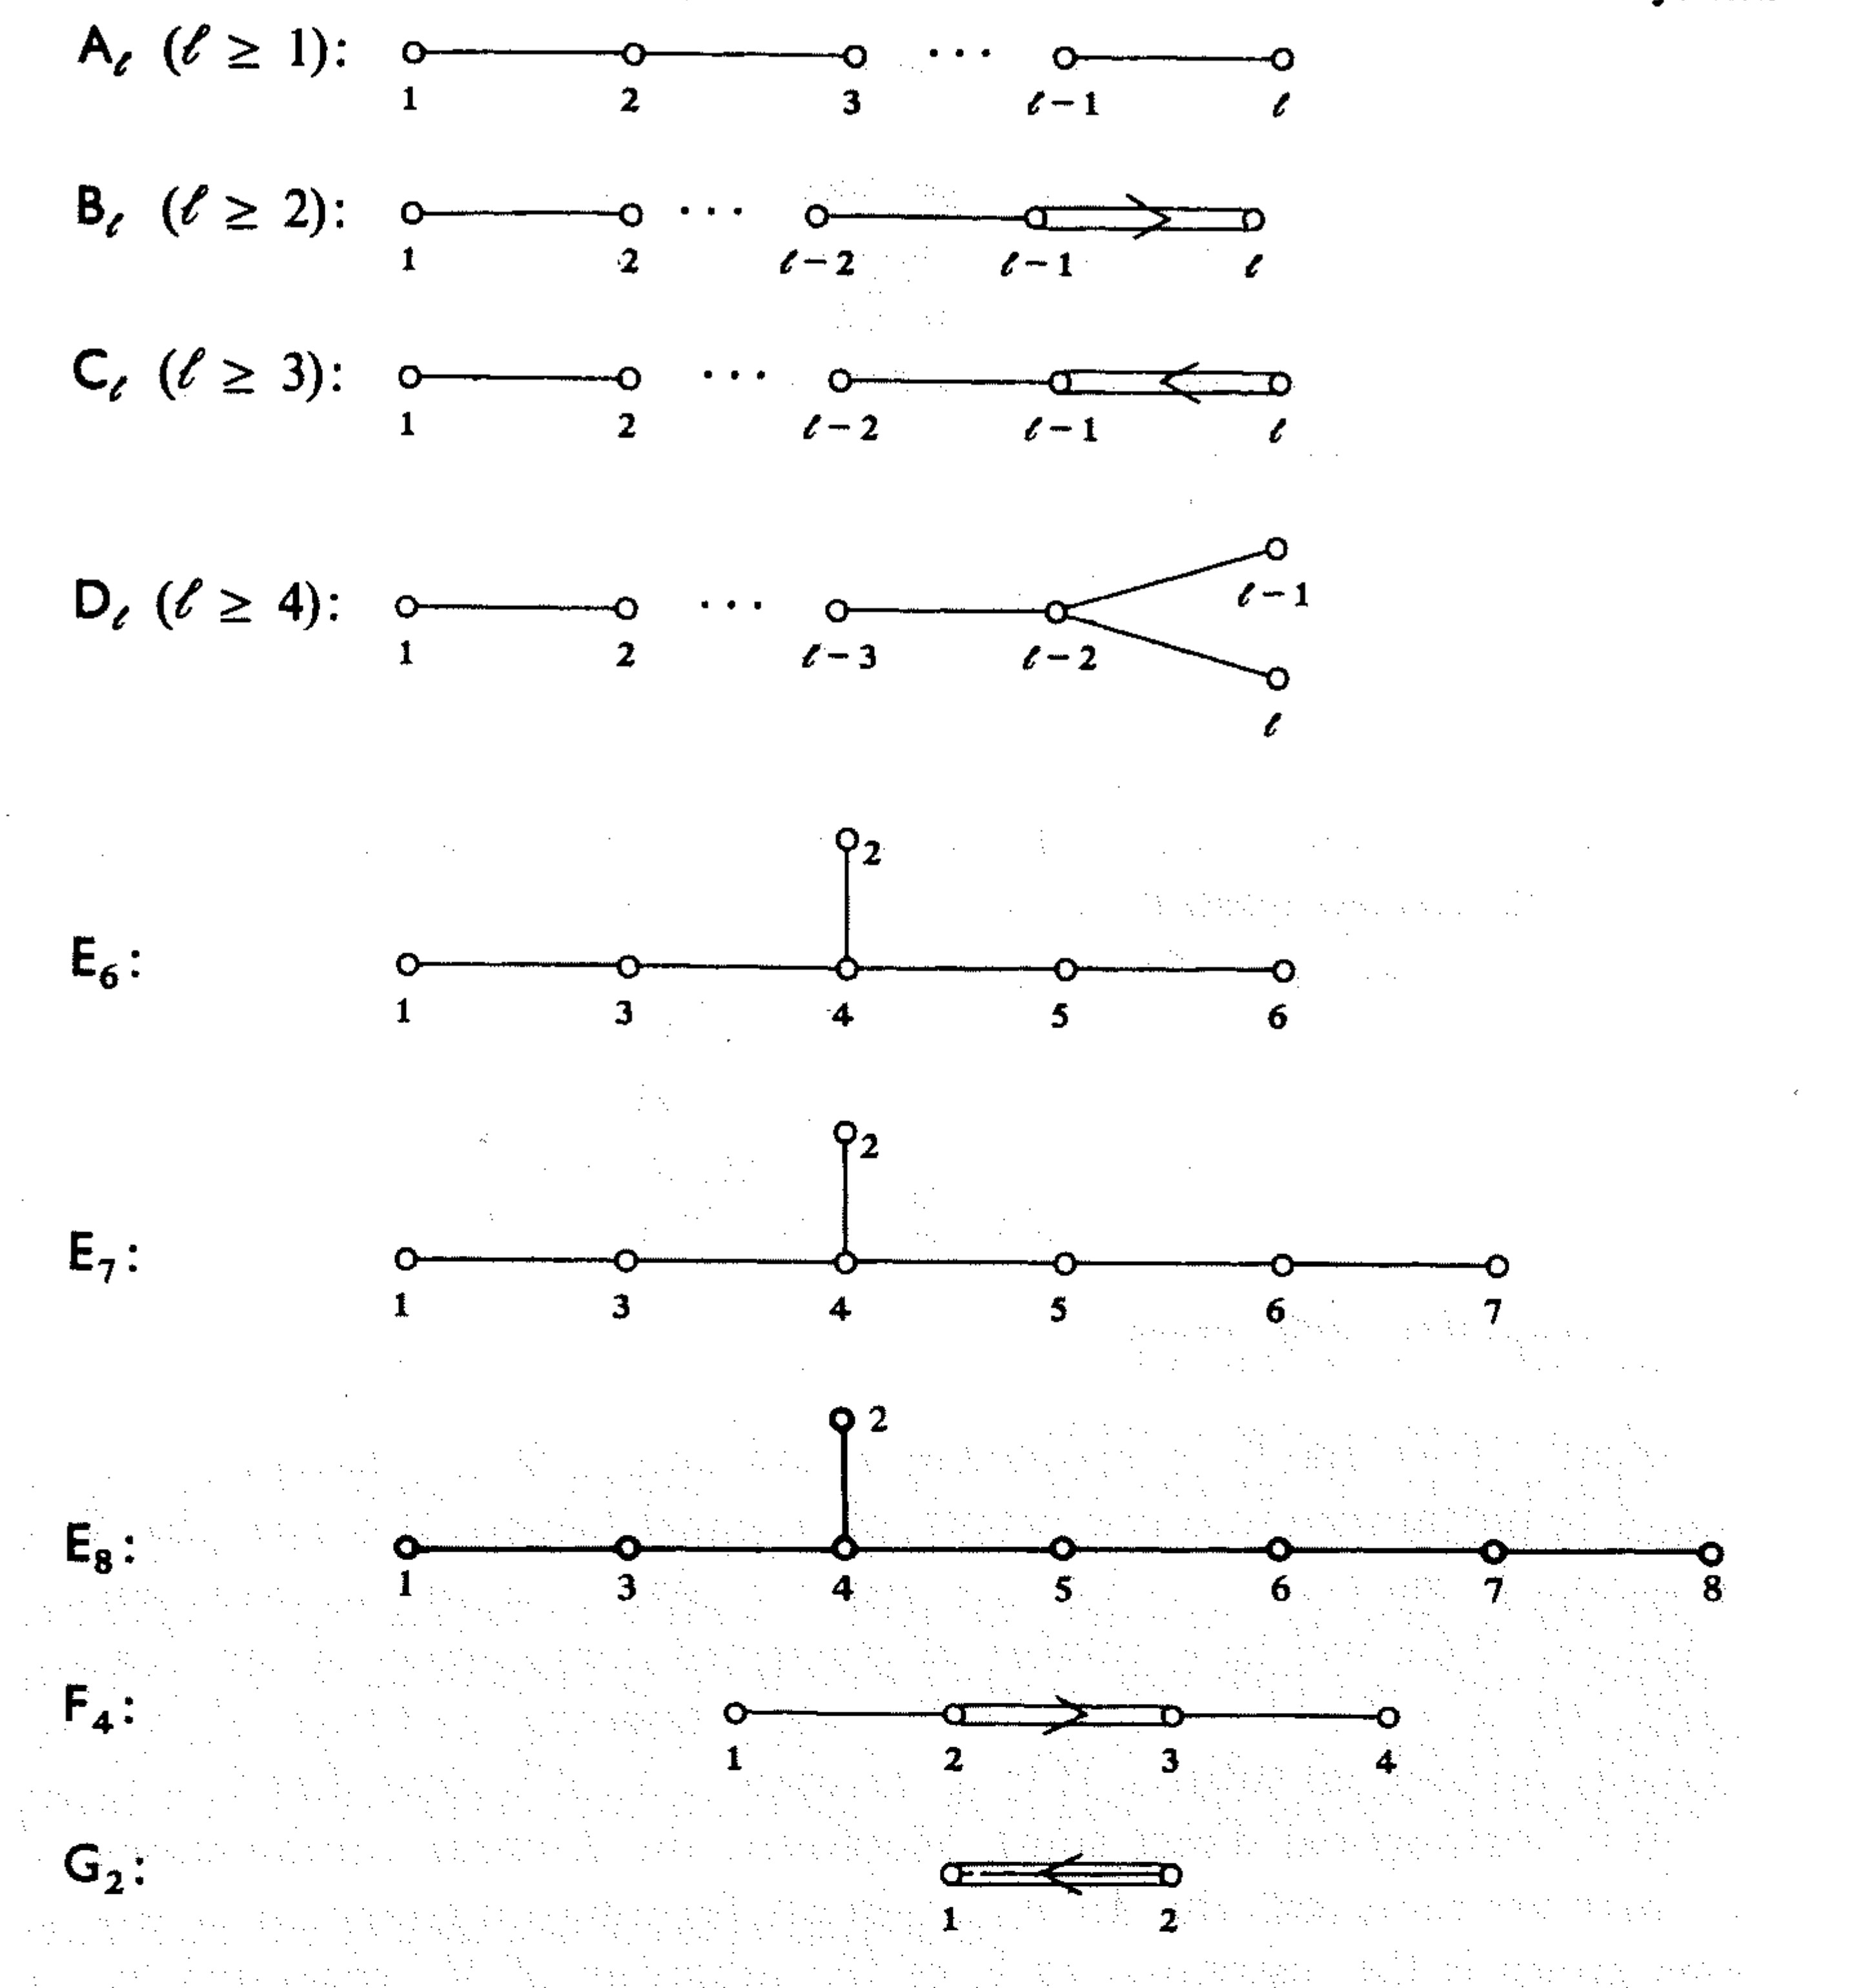
\includegraphics[width=0.8\textwidth]{00.jpg}
\end{figure}

\paragraph{Bemerkungen}
\begin{itemize}
\item Der Index $l$ wird eingeschränkt um Dopplungen zu vermeiden.
\item Man erkennt, dass abgesehen von $B_l$ und $C_l$ bereits die Coxeter Graphen ausreichen um die einfachen Wurzeln zu beschreiben.
\end{itemize}
\marginnote{47 min}

\subsubsection*{Beweis}
Wir werden nun die Coxeter Graphen klassifizieren und danach sehen, welche Dynkin-Diagramme sich daraus ergeben können. Wir ignorieren also zunächst die Längen der Wurzeln und können deshalb mit Einheitsvektoren arbeiten.

\paragraph{Definition}
Sei $E$ ein euklidischer Raum, $\mathcal{U} = \{ \epsilon_1, \ldots, \epsilon_n\} \subset E \quad$ $n$ linear unabhängige Einheitsvektoren. Wenn für $i \neq j$
\begin{framed}
\begin{align*}
(\epsilon_i,\epsilon_j) \leq 0 \quad \text{und} \quad 4(\epsilon_i, \epsilon_j)^2 = 0,\,1,\,2 \text{ oder } 3
\end{align*}
\end{framed}
gilt, nennen wir $\mathcal{U}$ zulässiges System (von Einheitsvektoren).\\
Zu einer zulässigen Menge ordnen wir wie oben den Graphen $\Gamma$ zu, bei dem die Vertices $i$ und $j$ ($i\neq j$) von $4(\epsilon_i,\epsilon_j)^2$ Kanten verbunden werden.

Wir wollen nun alle zusammenhängenden Graphen finden, die zu zulässigen Systemen gehören. Das sind offensichtlich genau die zusammenhängenden Coxeter-Graphen.
\marginnote{50 min}
\begin{enumerate}
\item Zunächst eine einfache Feststellung: \emph{Entfernt man aus einem zulässigen System einige $\epsilon_i$, bilden die Verbleibenden wieder ein zulässiges System. Den neuen Graphen erhält man, indem man die entsprechenden Vertices und alle dorthin zeigenden Kanten entfernt.}

\item \emph{Die Zahl von Vertexpaaren in $\Gamma$, die von mindestens einer Kante verbunden werden, ist $\lneq n$.}\\
Sei $\epsilon = \sum_{i=1}^n \epsilon_i$. Weil die $\epsilon_i$ linear unabhängig sind, folgt $\epsilon \neq 0$ und damit: 
\begin{align}
 0<(\epsilon,\epsilon) = n + 2 \sum_{i<j} (\epsilon_i, \epsilon_j)
 \label{Part2_01}
\end{align}
Sei nun $i,j$ ein Paar von Indices dessen Vertices verbunden sind, also:
\begin{align*}
&(\epsilon_i,\epsilon_j) \neq 0\\
\Rightarrow \quad &4(\epsilon_i,\epsilon_j)^2 = 1,\,2 \text{ oder } 3\\
\Rightarrow \quad &4(\epsilon_i,\epsilon_j)^2 \geq 1\\
\Rightarrow \quad &2|(\epsilon_i,\epsilon_j)| \geq 1\\
\Rightarrow \quad &2(\epsilon_i,\epsilon_j) \leq -1
\end{align*}
Wir erhalten also mit Ungleichung \eqref{Part2_01}, dass die Anzahl dieser Paare nicht größer als $n-1$ werden kann. 

\item \emph{$\Gamma$ enthält keine Kreise.}\\
Ein Kreis wäre der Graph $\Gamma'$ eines zulässigen Systems $\mathcal{U'} \subset \mathcal{U}$. $\mathcal{U'}$ würde gegen Punkt 2 des Beweises verstoßen.


\item \emph{Es können nicht mehr als 3 Kanten mit einer Vertex verbunden sein.}\\
Sei $\epsilon \in \mathcal{U}$ und $\eta_1, \ldots , \eta_k \in \mathcal{U}$ die paarweise verschiedenen Vektoren, die mit $\epsilon$ verbunden sind: 
\begin{align*}
(\epsilon,\eta_i) < 0 \text{ wobei } \{\epsilon, \eta_1, \ldots\} \text{ paarweise verschieden}
\end{align*}
Aus Punkt 3 des Beweises wissen wir, dass die $\eta_i$'s nicht miteinander verbunden sein können, also: $(\eta_i,\eta_j) = 0 $ für $i\neq j$.\\
Weil $\mathcal{U}$ linear unabhängig ist, können wir einen Einheitsvektor $\eta_0$ finden, der im Erzeugnis von $\mathcal{U}$ liegt und orthogonal zu allen $\eta_i$ ist. Damit kann $\eta_0$ nicht auch noch zu $\epsilon$ orthogonal sein: 
\begin{align}
(\epsilon,\eta_0) \neq 0
\label{Part4_01}
\end{align}

Es gilt nun:
\begin{align}
&\epsilon = \sum_{i=0}^k (\epsilon,\eta_i)\,\eta_i\notag\\
\Rightarrow\quad &1 = (\epsilon,\epsilon) =  \sum_{i=0}^k (\epsilon,\eta_i)^2\notag\\
\overset{\eqref{Part4_01}}{\Rightarrow} \quad & \sum_{i=1}^k (\epsilon,\eta_i)^2 < 1 \label{winkelabschaetzung} \\
\Rightarrow \quad & \sum_{i=1}^k 4(\epsilon,\eta_i)^2 < 4\notag
\end{align}
Die Gesamtzahl der Vertices, die mit $\epsilon$ verbunden sind, ist also strikt kleiner als 4.
\marginnote{59 min}

\item \emph{Der einzige zusammenhängende Graph eines zulässigen Systems, der eine Dreier-Kante enthält, ist der Graph $G_2$}\\
Die folgt sofort aus Punkt 4 des Beweises.

\item \emph{Sei $\{\epsilon_1, \ldots , \epsilon_k\} \subset \mathcal{U}$ eine Teilmenge, zu der eine einfache Kette gehört. Dann ist $\mathcal{U'} = ( \mathcal{U} \setminus \{\epsilon_1,\ldots,\epsilon_k \}) \cup \{\epsilon\}$ mit $\epsilon := \sum_{i=1}^k \epsilon_i$ ein zulässiges System. Man darf also eine einfache Kette zu einem Punkt zusammenschrumpfen.}\\
Wir müssen also zeigen, dass $\mathcal{U'}$ ein zulässiges System ist. Die lineare Unabhängigkeit ist klar. Nach Voraussetzung haben wir $2 (\epsilon_i, \epsilon_{i+1}) = -1 $ für alle $1\leq i\leq k-1$. Damit ist $\epsilon$ ein Einheitsvektor:
\begin{align*}
(\epsilon,\epsilon) = k + 2\sum_{i<j} (\epsilon_i,\epsilon_j) = k-2 \cdot\frac{k-1}{2} = 1
\end{align*}
Mit Punkt 3 des Beweises wissen wir, dass jedes $\eta \in \mathcal{U} \setminus \{\epsilon_1,\ldots, \epsilon_k  \}$ mit maximal einem $\epsilon_1,\ldots,\epsilon_k$ verbunden sein kann. Damit
\begin{align*}
(\eta,\epsilon) =0 \text{ oder } (\eta,\epsilon) = (\eta , \epsilon_i)  \quad 1\leq i\leq k
\end{align*}
Auf jeden Fall gilt $4(\eta, \epsilon)^2 = 0,\,1,\,2 \text{ oder } 3$.\\
Damit ist $\mathcal{U'}$ ein zulässiges System.
\marginnote{64 min}

\item \emph{$\Gamma$ enthält keinen Teilgraphen der folgenden Form:}
\begin{figure}[H]
\centering
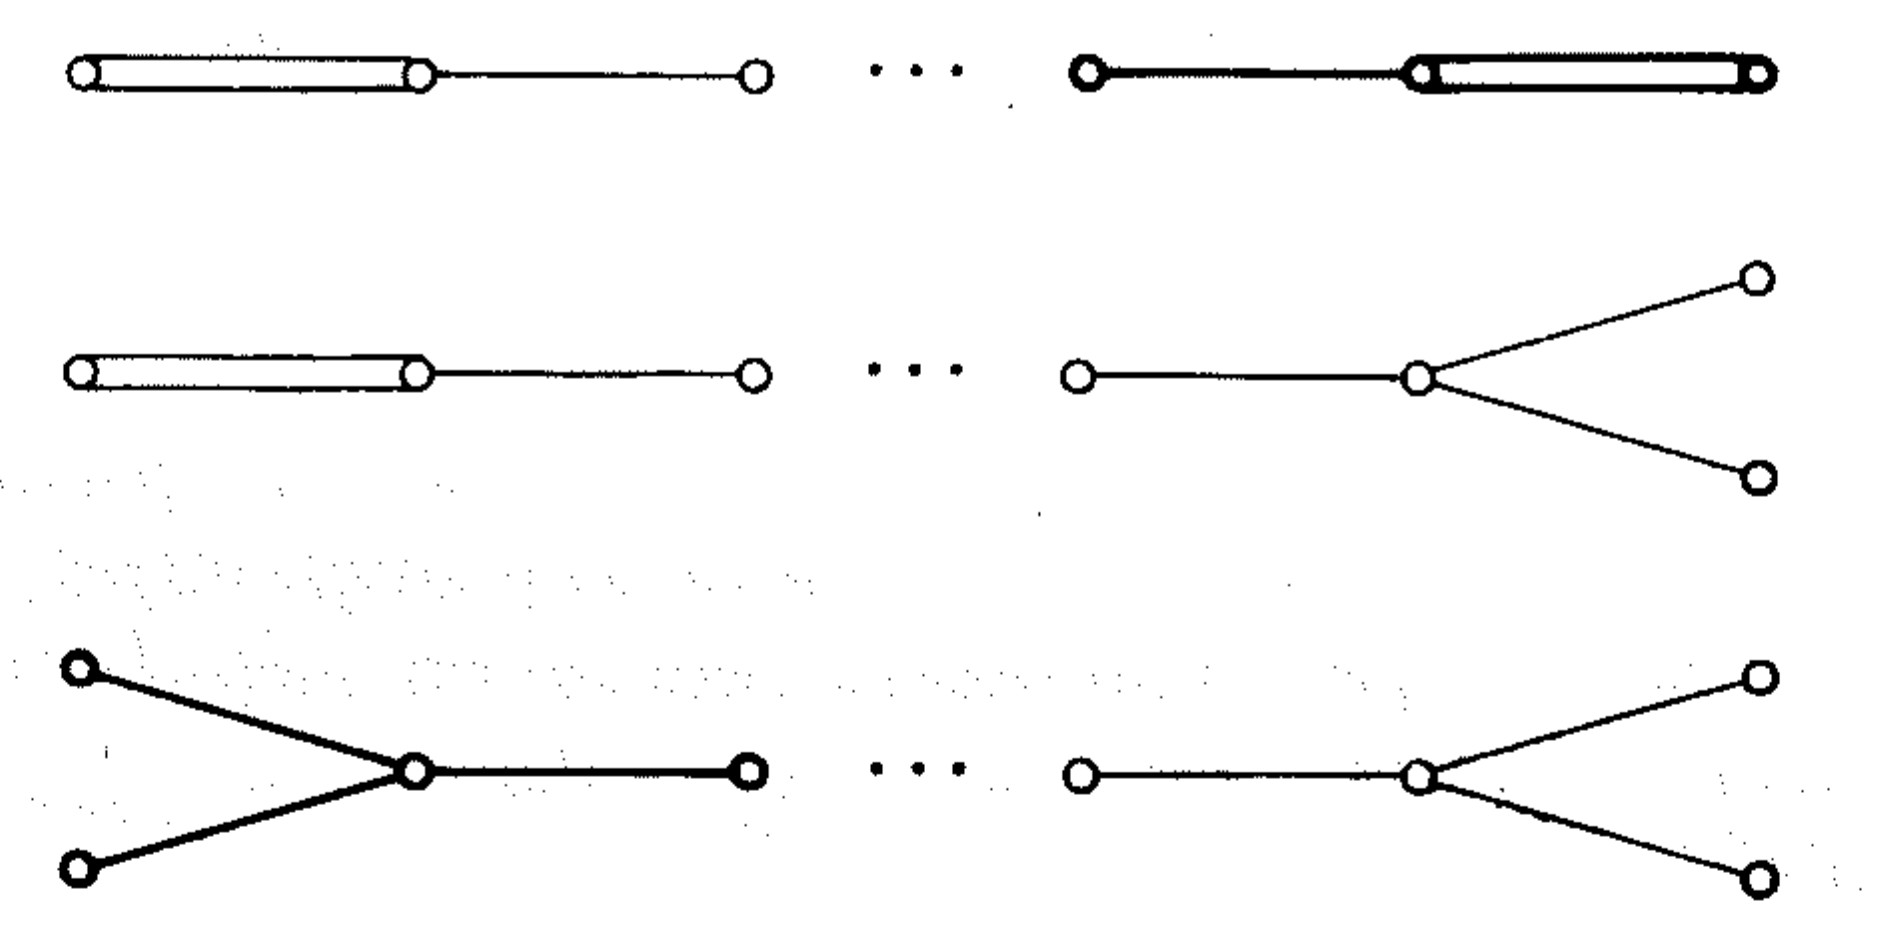
\includegraphics[width=0.3\textwidth]{71.jpg}
\end{figure}

Mit Punkt 1 des Beweises wissen wir, dass diese Graphen Teil eines zulässigen Systems wären. Punkt 6 erlaubt es die einfache Kette in der Mitte so zu entfernen, dass die entstehenden Graphen gegen Punkt 4 verstoßen.
\begin{figure}[H]
\centering
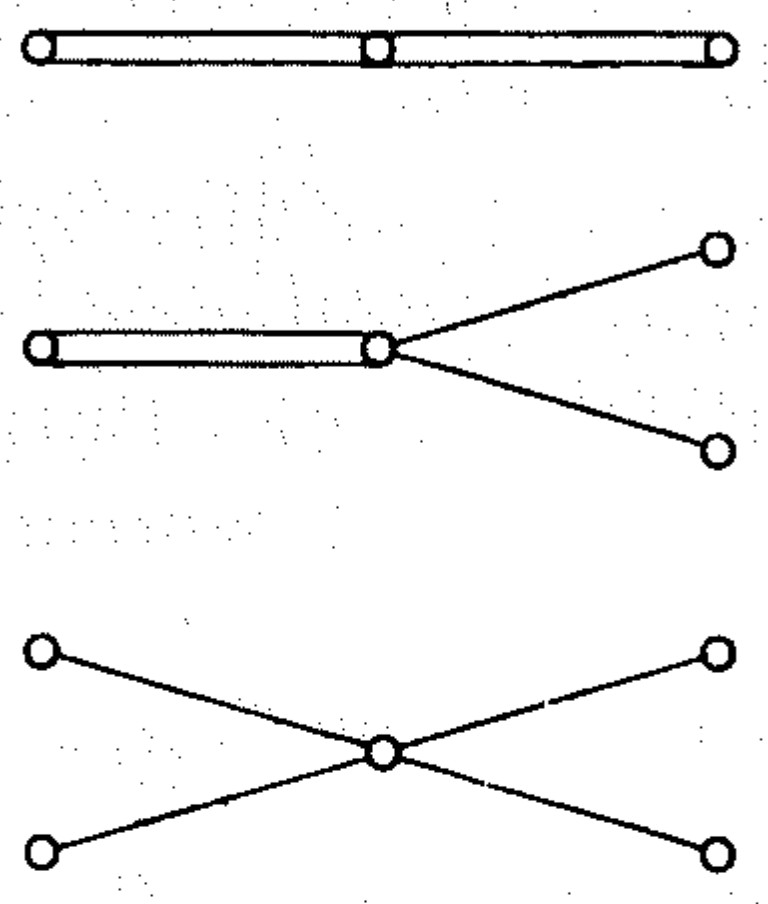
\includegraphics[width=0.1\textwidth]{72.jpg}
\end{figure}


\item \emph{Jeder Graph eines zulässigen Systems hat eine der folgenden Formen:}
\begin{figure}[H]
\centering
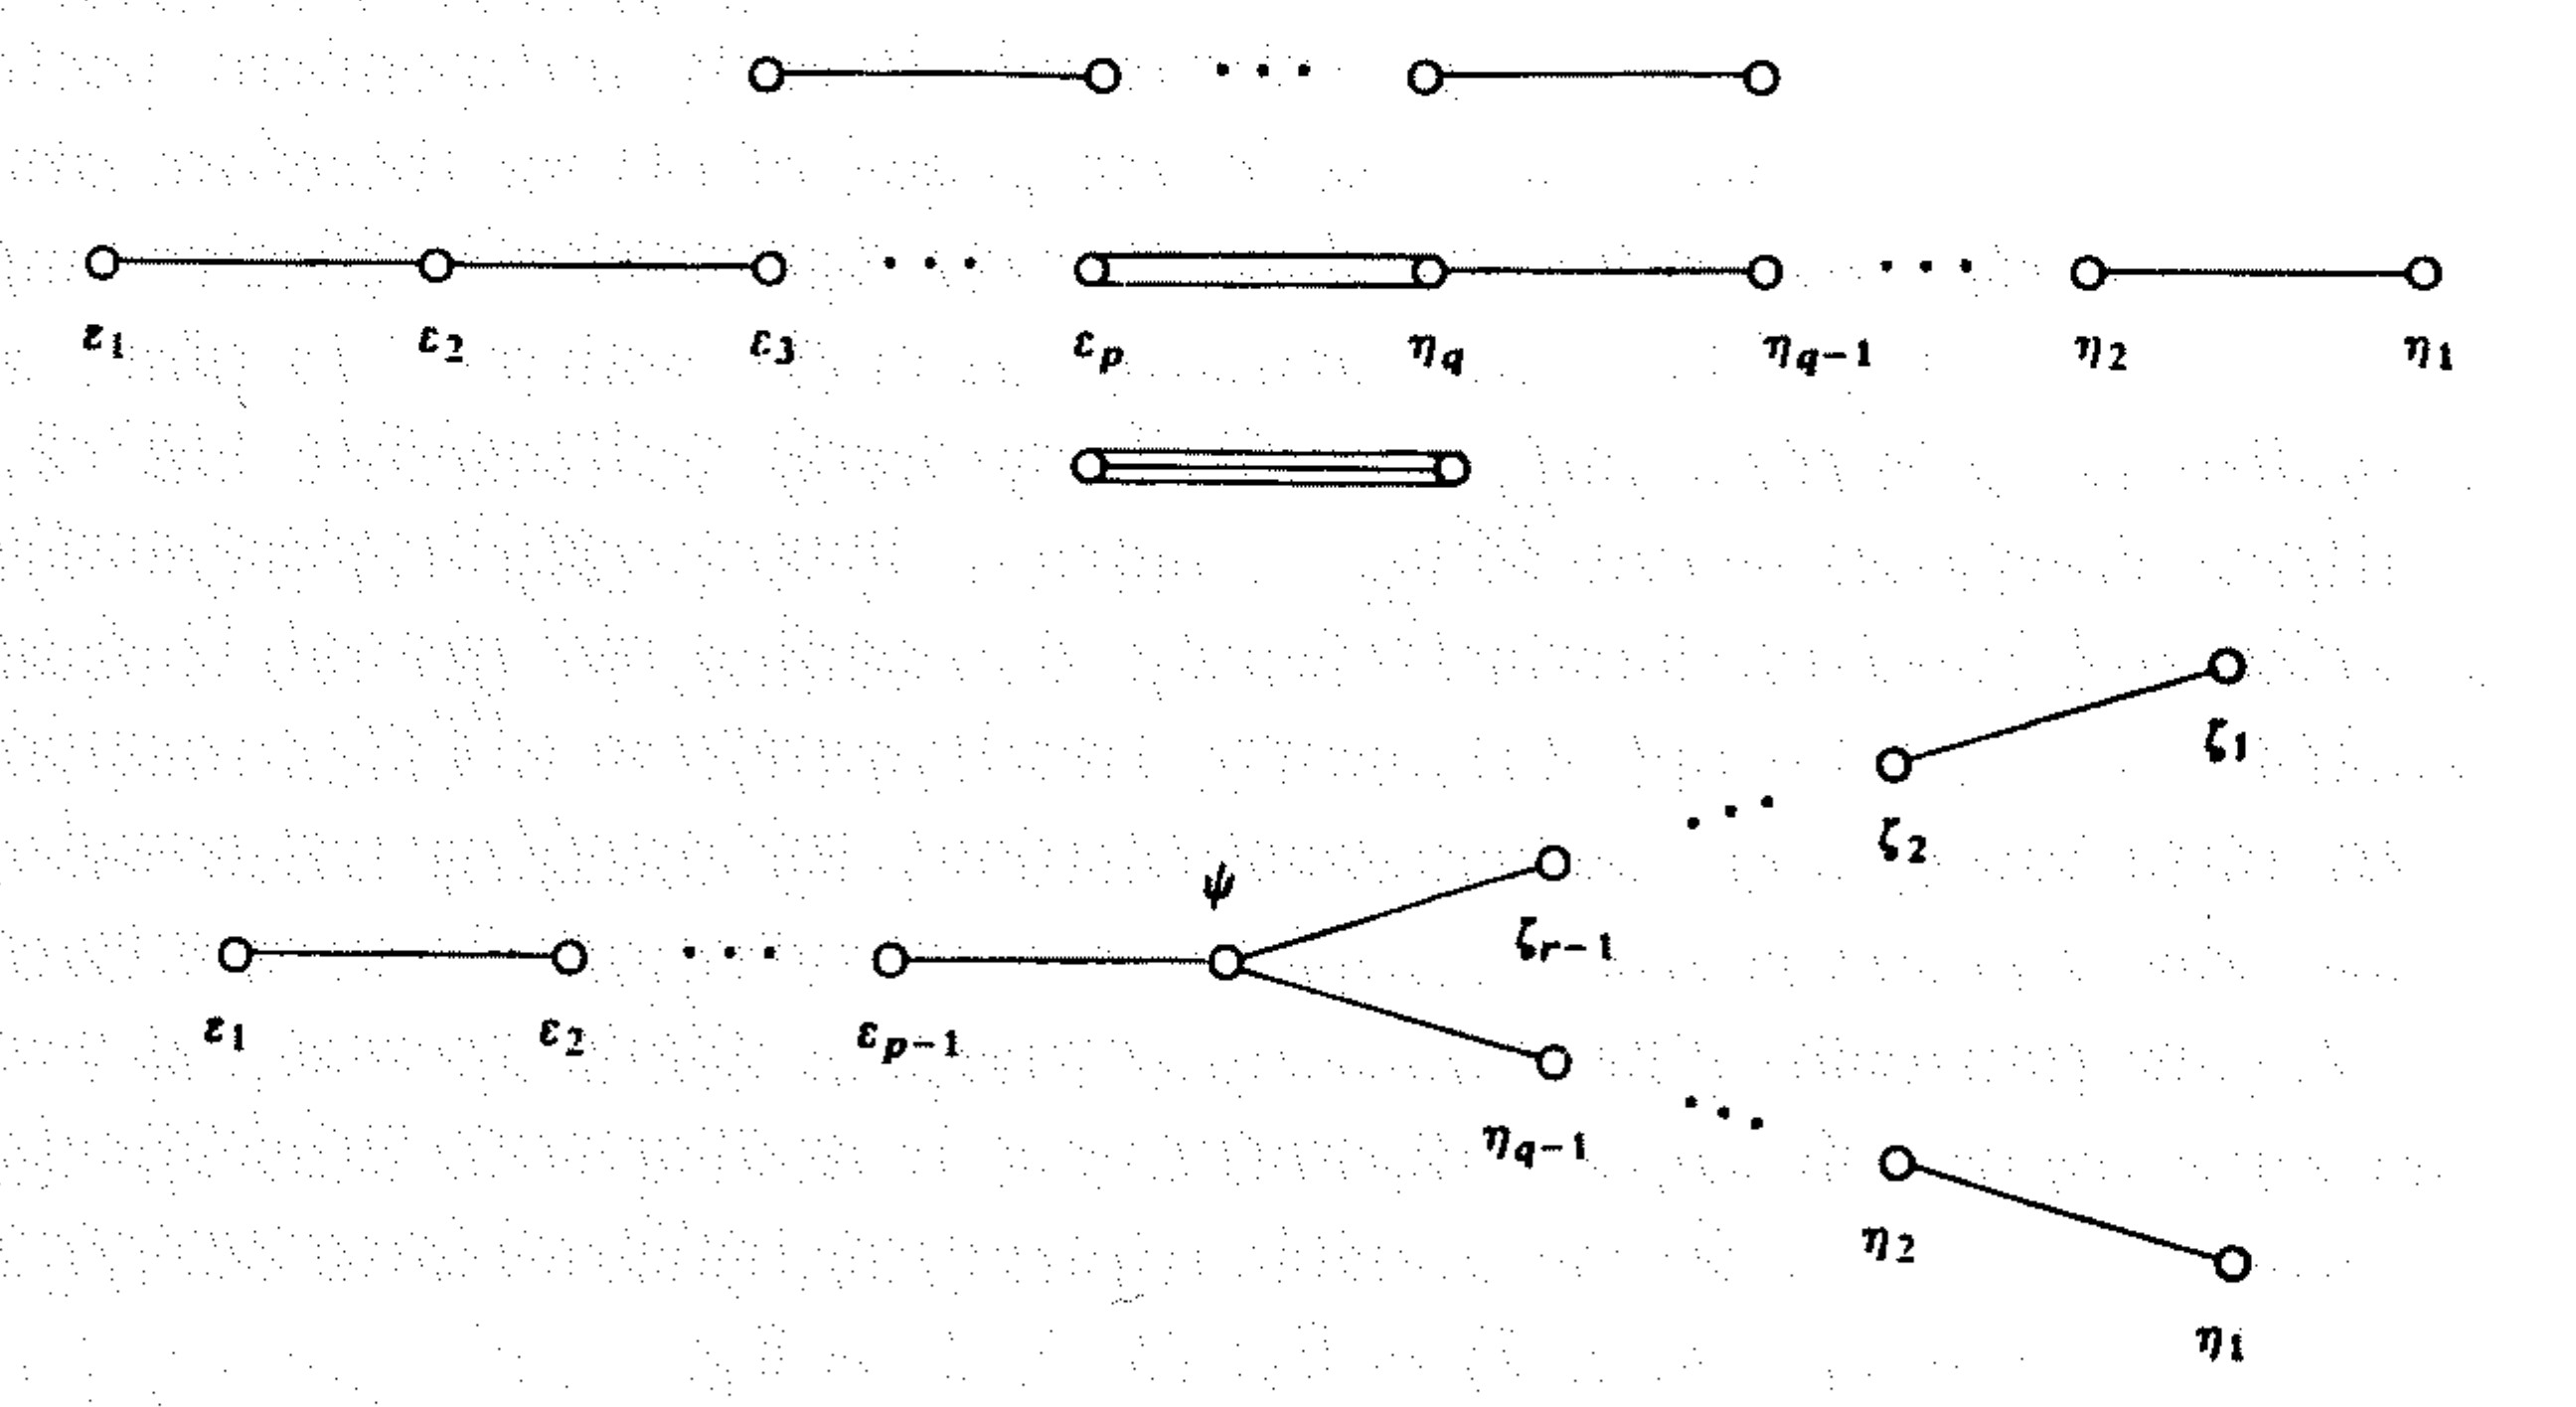
\includegraphics[width=0.8\textwidth]{81.jpg}
\end{figure}


\item \emph{Die einzigen zusammenhängenden Graphen des zweiten Typs in Punkt 8 sind der Coxeter Graph $F_4$ oder der Coxeter Graph $B_n (= C_n)$.}\\
Seien $\epsilon = \sum_{j=1}^p j\epsilon_j $ und $\eta = \sum_{j=1}^q j\eta_j$ mit $\epsilon_i, \eta_j$ wie in Punkt 8. Nach Voraussetzung $2(\epsilon_i, \epsilon_{i+1}) = -1 = 2(\eta_i, \eta_{i+1})$ und $(\epsilon_i, \eta_j) = 0$. Damit erhalten wir:
\begin{align}
&(\epsilon,\epsilon) = \sum_{j=1}^p j^2 - \sum_{j=1}^{p-1} j(j+1) = p(p+1)/2 \label{summationeps} \\
\text{und}\quad & (\eta,\eta) = q(q+1)/2\notag
\end{align}
Aus $4(\epsilon_p,\eta_q)^2 = 2$ können wir 
\begin{align*}
(\epsilon,\eta)^2 = p^2 q^2 (\epsilon_p, \eta_q)^2 = p^2 q^2 / 2
\end{align*}
folgern. Wir verwenden die Schwarzsche Ungleichung. Hier gilt sogar strikte Ungleichheit, weil $\epsilon$ und $\eta$ linear unabhängig sind. 
\begin{align*}
&(\epsilon,\eta)^2 < (\eta, \eta) (\epsilon,\epsilon)\\
\Rightarrow \quad& p^2q^2 / 2 < p(p+1)q(q+1)/4 =( p^2q^2 + pq^2 + p^2q+pq)/4 &|:(pq)\\
\Rightarrow \quad & 0<-pq+q+p+1& |\cdot (-1)\quad | +2\\
\Rightarrow \quad & 2>pq-q-p+1=(p-1)(q-1)
\end{align*}
Die Möglichkeiten diese Ungleichung zu erfüllen sein:
\begin{itemize}
\item $p=2=q:$ Dies ist der Fall $F_4$.
\item $p=2, q$ beliebig (oder umgekehrt): Hier liegt $B_l (= C_l)$ vor. 
\end{itemize}

\item \emph{Die einzigen Graphen vom vierten Typ in Punkt 8 sind die Coxeter-Graphen $E_6, E_7, E_8$ und $D_n$.}\\
Seien $\epsilon = \sum_{i=1}^{p-1} i\epsilon_i$, $\eta = \sum_{j=1}^{q-1} j\eta_j$ und $\zeta = \sum_{k=1}^{r-1} k \zeta_k$, wobei wir wieder die Notation aus Punkt 8 verwenden. $\epsilon, \eta$ und $\zeta$ sind linear unabhängig und orthogonal zueinander. $\psi$ liegt nicht in ihrem Erzeugnis.\\
Wie in Gleichung \eqref{winkelabschaetzung} erhalten wir
\begin{align*}
\cos ^2 \theta_1 + \cos ^2 \theta_2 + \cos ^2 \theta_ 3 < 1
\end{align*}
wobei $\theta_i$ die Winkel zwischen $\epsilon,\eta,\zeta$ und $\psi$ sind. \\
Aus der analogen Rechnung wie in Punkt 9 folgt ($p-1$ statt $p$ in Gleichung \eqref{summationeps})
\begin{align}
&(\epsilon,\epsilon) = p(p-1)/2\label{start} \\
\Rightarrow\quad & \cos ^2 \theta_1 = \frac{(\epsilon,\psi)^2}{(\epsilon,\epsilon)\underbrace{(\psi,\psi)}_{=1}}\notag\\
& = \frac{(p-1)^2 (\epsilon_{p-1},\psi)^2}{p(p-1)/2} = \frac{2(p-1)^2}{4p(p-1)}\notag\\
&= \frac{1}{2} \, \left( 1-\frac{1}{p} \right)\label{stop}
\end{align}
Diese Rechnungen (Gleichung \eqref{start} bis \eqref{stop}) laufen für $\eta$ und $\zeta$ analog. Insgesamt erhalten wir so: 

\begin{align*}
&\frac{1}{2} \left(  1-\frac{1}{p} + 1-\frac{1}{q} + 1-\frac{1}{r}   \right) <1
\end{align*}
\begin{framed}
\begin{align}
\Leftrightarrow \quad & \frac{1}{p} + \frac{1}{q} + \frac{1}{r} >1 \label{centraleq}
\end{align}
\end{framed}
Nach eventueller Umbenennung haben wir: $\frac{1}{p} \leq \frac{1}{q} \leq \frac{1}{r}$. Sind nun $p, q$ oder $r =1$ sind wir im Typ $A_n$. Ansonsten haben wir:
\begin{align}
& \frac{1}{p} \leq \frac{1}{q} \leq \frac{1}{r} \leq \frac{1}{2} \label{impoeq} 
\end{align}
Wir haben also 
\begin{align}
& 1\overset{\eqref{centraleq}}{<} 3\cdot \frac{1}{r} \overset{ \eqref{impoeq}}{\leq} 3\cdot\frac{1}{2	} \notag\\
\Rightarrow \quad & r=2\label{result_r}
\end{align}
Dies setzt auch Einschränkungen an $q$ (über \eqref{centraleq} und  \eqref{result_r}):
\begin{align}
&\frac{1}{p} + \frac{1}{q} >\frac{1}{2}\notag\\
\Rightarrow \quad & \frac{2}{q} > \frac{1}{2} \label{nealyqres} \\
\Rightarrow \quad & 2 \overset{\eqref{impoeq}}{\leq} q \overset{\eqref{nealyqres}}{<} 4\notag
\end{align}
Sei $q=3$. Dann ist $\frac{1}{p} >\frac{1}{6}$ und damit $p<6$.\\
Sei $q=2$. Dann ist $p$ beliebig.\\
Die erlaubten Tripel $(p,q,r)$ sind also: 
\begin{align*}
& (p,2,2) = D_n\\
& (3,3,2) = E_6\\
& (4,3,2) = E_7\\
& (5,3,2) = E_8
\end{align*}
\end{enumerate}

Außer in den Fällen $B_n, C_n$ legen die Coxeter-Graphen bereits eindeutig die Dynkin-Diagramme fest. Damit ist das Theorem gezeigt.
\hfill $\Box$\\
\marginnote{81 min}

\end{document}
